
\section{Global}
In each calculation of the global sensitivity analysis, the transition start 
time, percent of \glspl{LWR} operating for 80 years, the Xe-100 discharge 
burnup, \gls{MMR} burnup, and build share of one advanced reactor were 
varied. We decided to perform this analysis three separate times instead of 
varying all seven variables to prevent unwanted combinations of the 
advanced reactor build shares that result in large oversupplies or 
undersupplies of power. 

All of the variables included in this work can physically take any non-negative 
real value. However, the discharge burnup values used in this work are specific 
integer values. To reconcile the use of specific values when others are physical, 
we created surrogate models, similar to the ones used by Richards and Feng 
\cite{richards_application_2021}. We generated the data for the model by sampling 
across the input space 4500 times because the Dakota user's manual 
\cite{adams_dakota_2019} suggests running 

\begin{equation}
    100\times P\times(R+2)
\end{equation}

in which $P$ is the number of input parameters and $R$ is the number out response 
metrics. To assist in creation of the surrogate model, the \gls{MMR} burnup 
was converted from a discrete variable to a continuous variable by varying 
the lifetime of the reactor as need to achieve the burnup value. The 
\gls{MMR} burnup was restricted to between 41-90 MWd/kgU, the range 
for the values used in the other sensitivity analysis. 
The Xe-100 discharge burnup values were expanded as well, but remained 
a discrete variable. Additional burnup points were selected to represent 
between one and six passes for each pebble with a residence time of six, seven, 
or eight months for each pass. This expansion of the Xe-100 burnup resulted 
in 16 different burnup values between 28-185 MWd/kgU. The other variables were 
only restricted to the specified range previously used for the variable (e.g., 
0-50\% for the \gls{LWR} lifetime extensions) and were treated as continuous 
variables.
We randomly sampled (using the Latin Hypercube Sampling 
method in Dakota) each continuous variable based on the possible values and 
calculated the metrics for these samples. This data was then used to create 
the surrogate model to perform the global sensitivity analysis and 
calculate the Sobol' indices. 

When creating the surrogate model we once again used random sampling for all 
of the variables, but allowed all of the input parameters to be continuous 
variables. 
We used both the gaussian and quadratic fits to the data 
to create the surrogate models, similar to what Richards and 
Feng did \cite{richards_application_2021}. 
We also instructed Dakota to perform variance decomposition 
on the surrogate model so that Sobol' indices would be calculated. The 
results presented in this section are the Sobol' indices that describes the 
impact of each input parameter on each output metric. The total and the main 
Sobol' indices are reported, which describe the contribution from the parameter 
and its interactions with all of the other parameters and the contribution from 
just the parameter, respectively. 

\subsection{Scenario 7}

\subsubsection{Xe-100 build share}
When running the gaussian surrogate model for the variations in the Xe-100 build 
share, the models all  have an R$^2$ value of 1, which means that the outputs of 
the surrogate models match perfectly to the data provided from the initial 
\Cyclus runs. The large R$^2$ value suggests that this surrogate model type 
fits to noise in the data provided. A comparison of the results of the 
gaussian surrogate model and the data provided to the model shows some interesting 
results. Figure \ref{fig:s7_xe100_gaussian} compares the values of the
\gls{HALEU} mass as a function of the Xe-100 burnup for the Gaussian model 
and the input data. The results of the Gaussian model follows the input 
data well, nearly reaching the maximum and minimums of the data. However, 
closer inspection of the data shows that results of the Gaussian model 
include non-physical results, such as negative values of \gls{HALEU} mass. 
These values suggest that the Gaussian model is extrapolating some, instead 
of just interpolating. Therefore, the Gaussian model is not a perfect 
match to the input data, which means that the Sobol' indices are different 
than if the variance decomposition were performed on the input data. 

\begin{figure}
    \centering 
    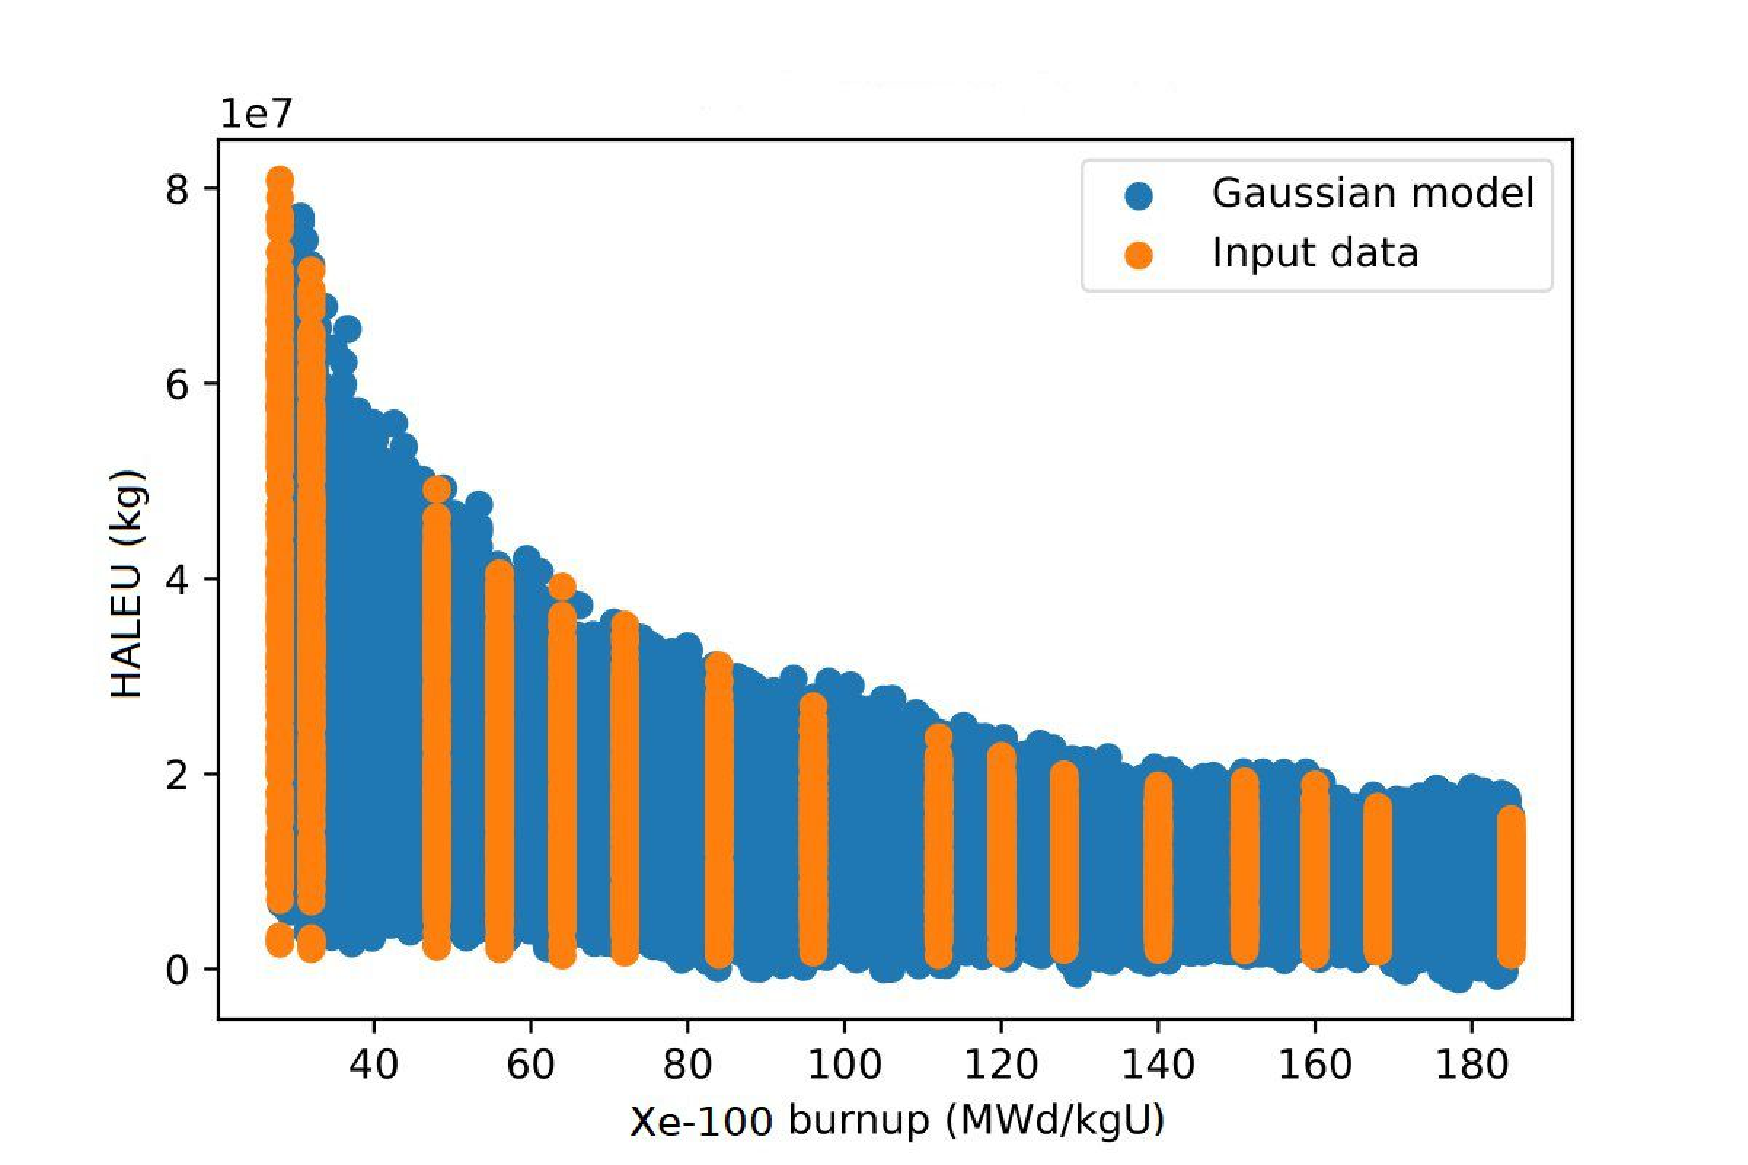
\includegraphics[scale=0.8]{xe100_share_gaussian_xe100_burnup_haleu.pdf}
    \caption{Comparison of the input data and the results of the gaussian 
    surrogate model when the Xe-100 build share is varied. }
    \label{fig:s7_xe100_gaussian}
\end{figure}

Table \ref{tab:s7_sobol_xe100_gaussian} reports the main and total Sobol' indices 
for each input parameter on each output metric. The highlighted cells have 
a total Sobol' index of at least 0.5. The Xe-100 build share and Xe-100 
burnup have the largest Sobol' indices for most of the output metrics. 

The \gls{MMR} burnup has a small Sobol' index for all of the output metrics
because a very small portion of the fleet are \glspl{MMR}. The Xe-100 build share 
does not have as much of an impact on the total \gls{SWU} capacity, compared 
with its impact on the other metrics, because of the similar \gls{SWU} 
capacity required by the Xe-100 and the VOYGR, and the replacement of Xe-100s 
with VOYGRs as the Xe-100 build share decreases. The transition start time 
has little effect on any of the metrics, which is consistent with the 
results of the \gls{OAT} and synergistic analysis. The \gls{LWR} lifetimes 
do not greatly affect any of the \gls{HALEU}-related metrics or the 
total \gls{SWU} capacity. This parameter has some impact on the total 
fuel mass and the \gls{SNF} mass, but less of an impact than the Xe-100 
build share. 

The Xe-100 build share has the largest impact on the \gls{SNF} mass, and 
the other parameters do not have much of an impact. This parameter 
has more of an impact on the \gls{SNF} mass than the other parameters because 
of the replacement of Xe-100s with VOYGRs as the Xe-100 build share decreases. 
The VOYGR 

\begin{table}
    \centering
    \caption{Sobol' indices for the Gaussian model when varying the 
    Xe-100 build share. The first value is the 
    main index, the second value is the total index.}
    \label{tab:s7_sobol_xe100_gaussian}
    \begin{tabular}{c c c c c c c}
        \hline
        & \multicolumn{6}{c}{Output Metric} \\
        Parameter & Fuel Mass & HALEU Mass & SWU & HALEU SWU & Feed & SNF Mass \\
        \hline
        Transition Start & 0.003/0.003 & 0.007/0.007 & 0.007/0.009 &
                           0.009/0.009 & 0.006/0.009 & 0.003/0.003\\
        LWR Lifetime & 0.268/0.280 & 0.012/0.021 & 0.081/0.095 &
                       0.013/0.022 & 0.013/0.022 & 0.301/0.314\\
        Xe-100 Build Share & \cellcolor{green!25}0.478/0.533 & \cellcolor{green!25}0.375/0.513 & 0.099/0.283 &
        \cellcolor{green!25}0.374/0.511 & \cellcolor{green!25}0.374/0.512 & 0.411/0.474\\
        Xe-100 Burnup & 0.188/0.247 & \cellcolor{green!25}0.465/0.571 & \cellcolor{green!25}0.622/0.775 & 
        \cellcolor{green!25}0.463/0.568 & \cellcolor{green!25}0.463/0.568 & 0.214/0.280\\
        MMR Burnup & 0.002/0.002 & 0.003/0.004 & 0.005/0.006 & 
                     0.004/0.005 & 0.004/0.005 & 0.002/0.002\\
        \hline        
    \end{tabular}
\end{table}

When using a quadratic surrogate model, the R$^2$ values for the training points on 
each output metric range between 0.921-0.966. Therefore, these model are still expected to 
fit the input data provided but not be fit to the noise in the input data 
as much as the Gaussian models. A comparison of the Xe-100 burnup and \gls{HALEU} 
mass for the input data and the results of the quadratic model (Figure 
\ref{fig:s7_xe100_quadratic}) shows that the quadratic model does 
capture the overall trend of the input data. However, like the Gaussian model, 
the quadratic model gives the non-physical result of a negative mass. Additionally, 
the results of the quadratic model do not meet the maximum of the input data and 
provide multiple results below the minimum value of the input data. Therefore, 
the quadratic model is also performing some extrapolation of the data based on the 
fit placed on the data.

\begin{figure}
    \centering 
    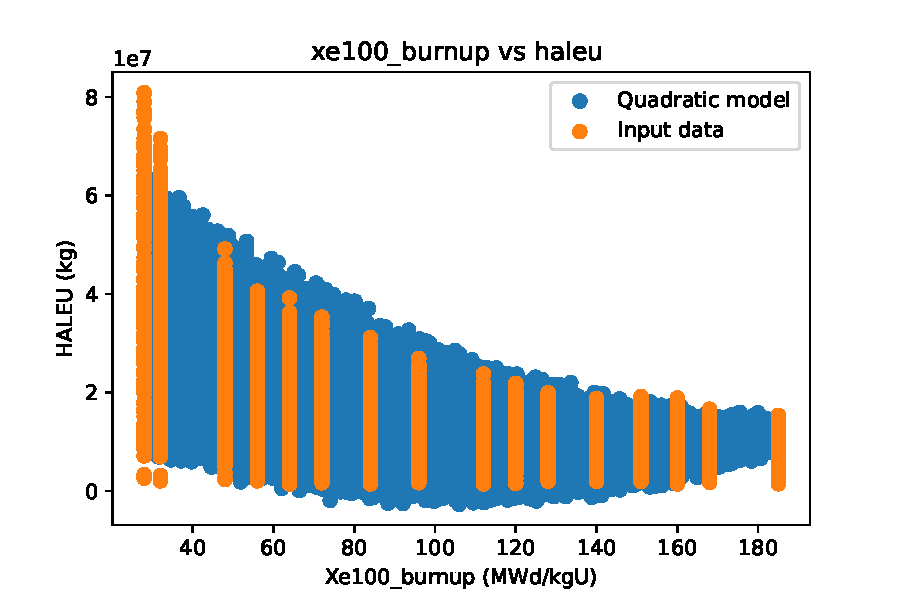
\includegraphics[scale=0.8]{xe100_share_quadratic_xe100_burnup_haleu.pdf}
    \caption{Comparison of the input data and the results of the gaussian 
    surrogate model when the Xe-100 build share is varied.}
    \label{fig:s7_xe100_quadratic}
\end{figure}

The Sobol' indices for each input parameter on each metric from the quadratic 
surrogate model are shown in Table \ref{tab:s7_sobol_xe100_quadratic}. The 
green cells identify total Sobol' indices that are at least 0.5. The same patterns 
observed in the Sobol' indices from the Gaussian model are 
observed in the values from the quadratic model as well. The Xe-100 build share 
and Xe-100 burnup affect the metrics the most, the \gls{LWR} lifetime has some 
impact, and the \gls{MMR} burnup and transition start time has the smallest impact 
on the metrics. 

\begin{table}
    \centering
    \caption{Sobol' indices for the quadratic model when varying the Xe-100 
    build share. The first number is the main index, the second is the total 
    index.}
    \label{tab:s7_sobol_xe100_quadratic}
    \begin{tabular}{c c c c c c c}
        \hline
        & \multicolumn{6}{c}{Output Metric} \\
        Parameter & Fuel Mass & HALEU Mass & SWU & HALEU SWU & Feed & SNF Mass \\
        \hline
        Transition Start & 0.000/0.000& 0.006/0.005 & 0.007/0.007 &
                           0.008/0.007 & 0.008/0.007 & 0.002/0.004\\
        LWR Lifetime & 0.278/0.286 & 0.014/0.021 & 0.082/0.089 & 
                       0.015/0.022 & 0.015/0.022 & 0.310/0.319\\
        Xe-100 Build Share & \cellcolor{green!25}0.443/0.501 & \cellcolor{green!25}0.374/0.500 & 0.115/0.283 & 
                             0.374/0.499 & 0.374/0.499 & 0.375/0.441\\
        Xe-100 Burnup & 0.214/0.279 & \cellcolor{green!25}0.472/0.578 & \cellcolor{green!25}0.624/0.773 &
                        \cellcolor{green!25}0.470/0.576 & \cellcolor{green!25}0.430/0.576 & 0.243/0.315\\
        MMR Burnup & 0.001/0.001 & 0.002/0.002 & 0.004/0.004 &
                     0.003/0.003 & 0.003/0.003 & 0.001/0.001\\
        \hline        
    \end{tabular}
\end{table}

Based on the results from each model, the Xe-100 build share and Xe-100 burnup 
should be varied to have the largest impact on the metrics

\subsubsection{MMR build share}
The Gaussian model has an R$^2$ value of 1 with respect to each of the output 
metrics. This value means that these models are also expected to fit the input 
data very well, including any noise present in the data. As Figure 
\ref{fig:s7_mmr_gaussian} shows, the data from the Gaussian model fits well 
to the input data provided. Unlike the models predicted based on input data when 
the Xe-100 build share was varied, this model does not result in any negative 
mass values. However, it still results in mass values lower than what is 
present in the input data which suggests that this model also extrapolates 
on some of the data. 

\begin{figure}
    \centering 
    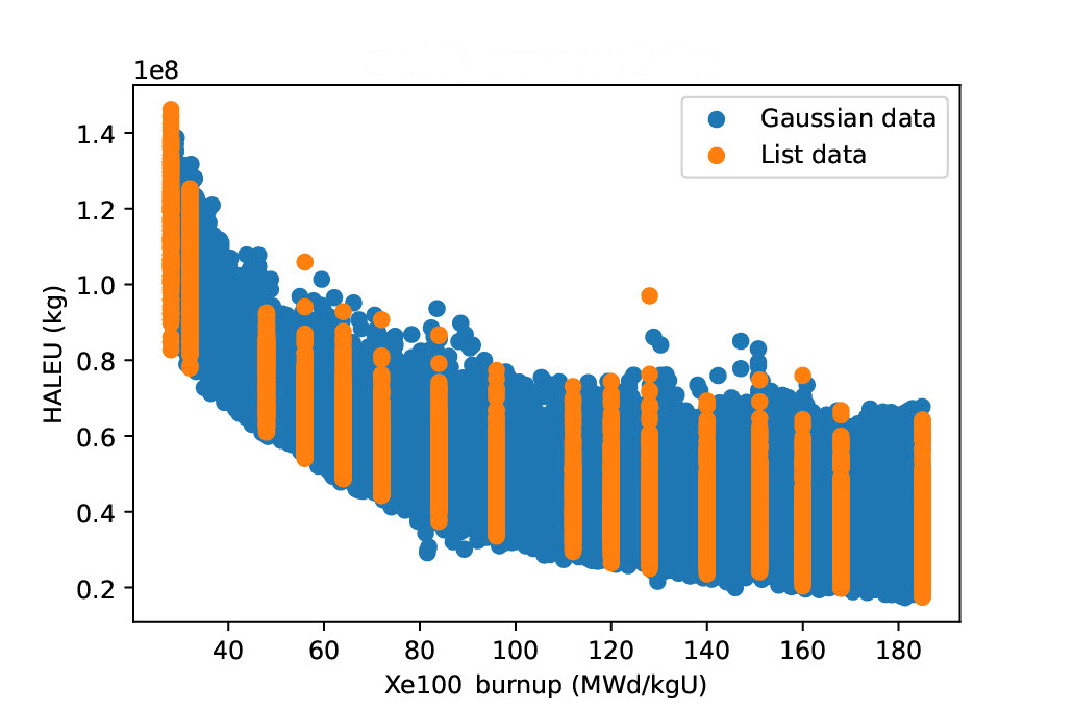
\includegraphics[scale=0.8]{mmr_share_gaussian_xe100_burnup_haleu.pdf}
    \caption{Comparison of the input data and the results of the Gaussian 
    surrogate model when the MMR build share is varied.}
    \label{fig:s7_mmr_gaussian}
\end{figure}

Examination of the Sobol' indices for this model (Table \ref{tab:s7_sobol_mmr_gaussian})
shows that the Xe-100 burnup has the largest impact on all of the 
output metrics. This is somewhat surprising, as one may expect the \gls{MMR} 
build share and \gls{MMR} burnup to have a strong combined impact on 
the results. However, this result is consistent with the results 
shown for the synergistic analysis (Figures \ref{fig:mmr_share_xe100_burnup} and 
\ref{fig:mmr_share_mmr_burnup}). When the Xe-100 burnup was varied on combination 
with the \gls{MMR} share, the range of values for each metric was larger than 
when the \gls{MMR} burnup was varied with the \gls{MMR} build share. 

Similar to the results from varying the Xe-100  build share, the 
transition start time has no impact on the results. The \gls{LWR} 
lifetime has less of an impact on the metrics than when the Xe-100 
build share was varied. The \gls{MMR} has almost no impact on the 
output metrics. 

\begin{table}
    \centering
    \caption{Sobol' indices for the Gaussian model when varying the MMR 
    build share. The first number is the main index, the second is the total 
    index.}
    \label{tab:s7_sobol_mmr_gaussian}
    \begin{tabular}{c c c c c c c}
        \hline
        & \multicolumn{6}{c}{Output Metric} \\
        Parameter & Fuel Mass & HALEU Mass & SWU & HALEU SWU & Feed & SNF Mass \\
        \hline
        Transition Start & 0.001/0.006 & 0.000/0.004 & 0.001/0.001 &
                           0.001/0.001 & 0.001/0.001 & 0.001/0.006\\
        LWR Lifetime & 0.054/0.068 & 0.047/0.063 & 0.055/0.071 &
                       0.054/0.069 & 0.054/0.069 & 0.057/0.071\\
        MMR Build Share & 0.069/0.107 & 0.068/0.107 & 0.162/0.203 &
                          0.162/0.204 & 0.152/0.193 & 0.015/0.055\\
        Xe-100 Burnup & \cellcolor{green!25}0.806/0.846 & \cellcolor{green!25}0.819/0.858 & \cellcolor{green!25}0.700/0.732 &
        \cellcolor{green!25}0.701/0.734 & \cellcolor{green!25}0.713/0.747 & \cellcolor{green!25}0.858/0.900\\
        MMR Burnup & 0.035/0.049 & 0.037/0.050 & 0.054/0.071 &
                     0.054/0.071 & 0.052/0.069 & 0.038/0.053\\
        \hline        
    \end{tabular}
\end{table}

When using the quadratic surrogate model, the models have R$^2$ values of 0.94
with respect to each of the output metrics. Therefore, these models also fit 
the data well without fitting all of the noise present in the input data. 
As Figure \ref{fig:s7_mmr_quadratic} shows, the output of the quadratic model 
fits the input data well, but not perfectly. Similar to the quadratic 
model created from varying the Xe-100 build share, this model 
does not perform well in fitting the maximum values and under-predicts 
some of the minimum values in the input data. 

\begin{figure}
    \centering 
    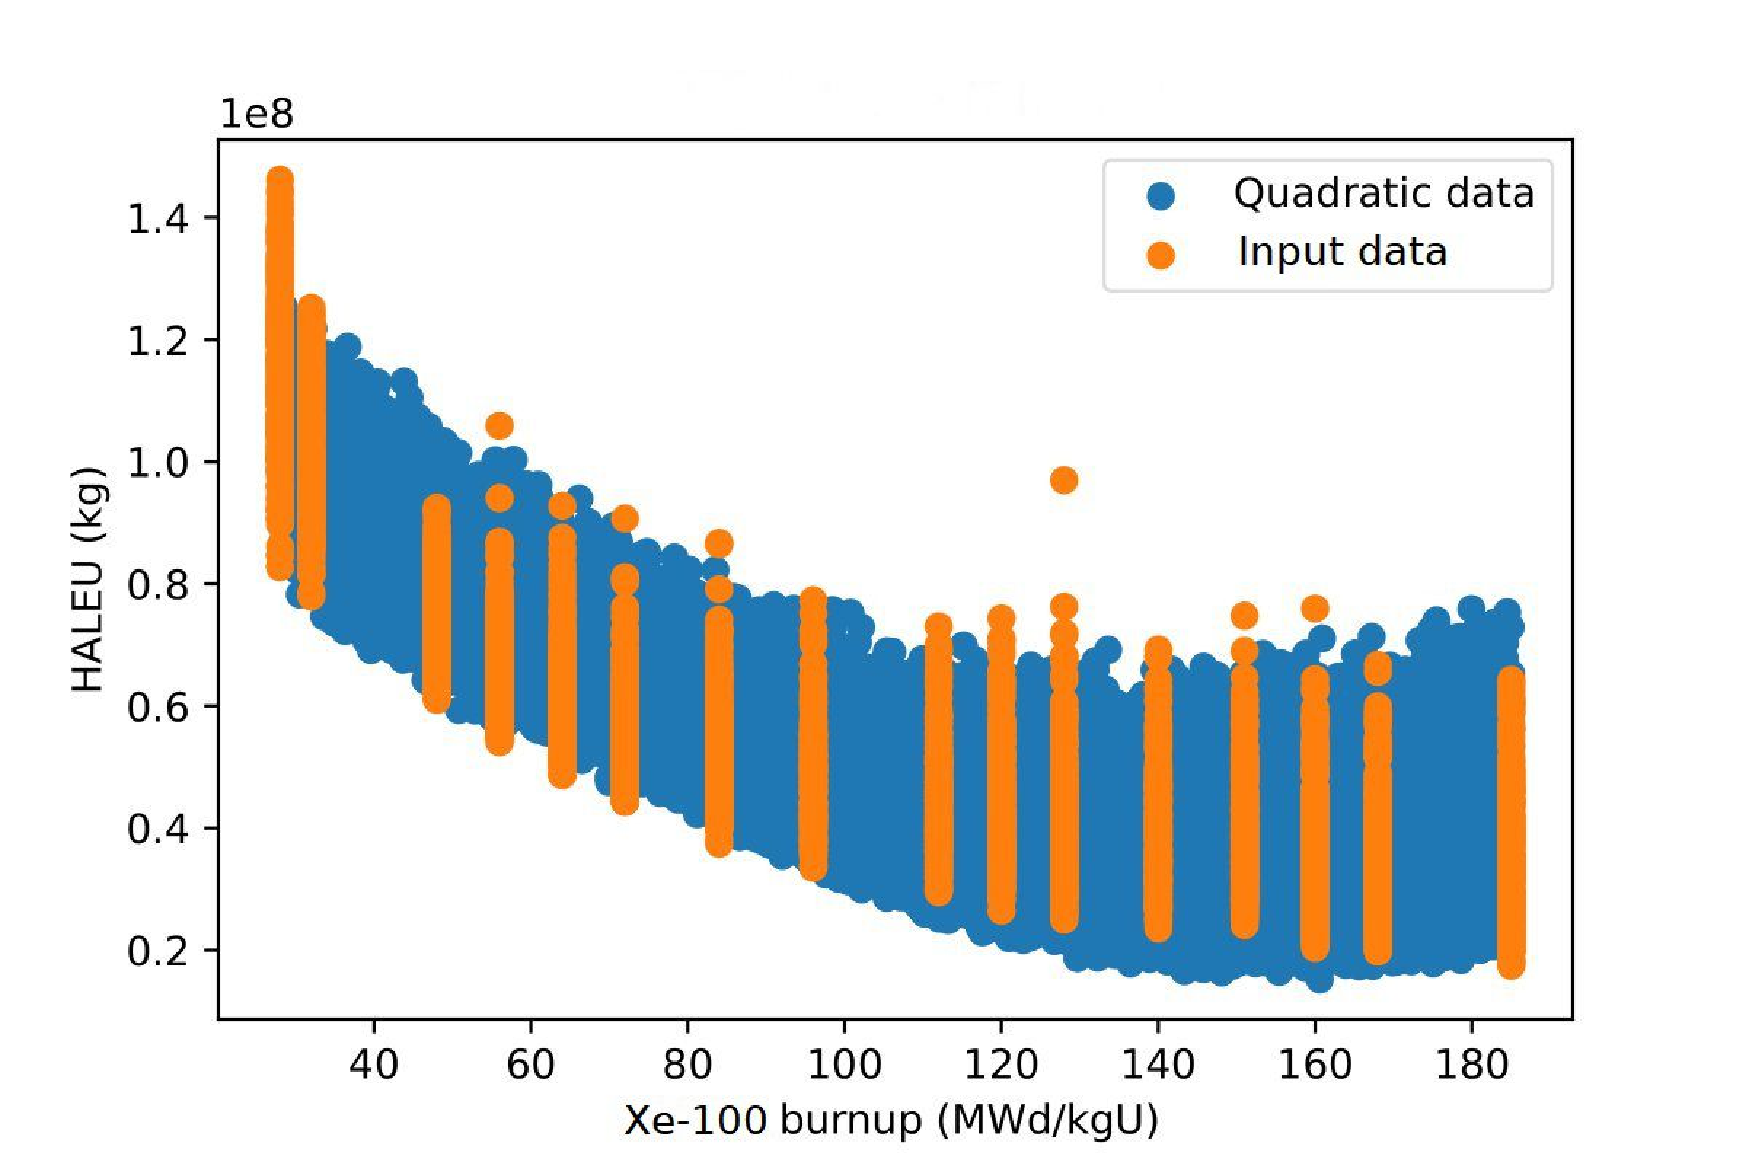
\includegraphics[scale=0.8]{mmr_share_quadratic_xe100_burnup_haleu.pdf}
    \caption{Comparison of the input data and the results of the quadratic 
    surrogate model when the MMR build share is varied.}
    \label{fig:s7_mmr_quadratic}
\end{figure}

The Sobol' indices from the quadratic model are similar to those from the 
Gaussian model. The Xe-100 burnup has the largest impact on all of the 
output metrics. The \gls{MMR} build share has the next largest impact 
on the metrics, but it is a very small impact. The other model 
parameters have a negligible effect on the metrics. 

\begin{table}
    \centering
    \caption{Sobol' indices for the quadratic model when varying the MMR 
    build share. The first number is the main index, the second is the total 
    index.}
    \label{tab:s7_sobol_mmr_quadratic}
    \begin{tabular}{c c c c c c c}
        \hline
        & \multicolumn{6}{c}{Output Metric} \\
        Parameter & Fuel Mass & HALEU Mass & SWU & HALEU SWU & Feed & SNF Mass \\
        \hline
        Transition Start & 0.002/0.003 & 0.000/0.000 & 0.000/0.000 &
                        0.000/0.000 & 0.000/0.000 & 0.002/0.003\\
        LWR Lifetime & 0.023/0.062 & 0.046/0.054 & 0.050/0.059 &
                       0.049/0.057 & 0.049/0.057 & 0.054/0.064\\
        MMR Build Share & 0.051/0.087 & 0.052/0.089 & 0.133/0.171 &
                          0.133/0.171 & 0.124/0.162 & 0.008/0.046\\
        Xe-100 Burnup & \cellcolor{green!25}0.834/0.866 & \cellcolor{green!25}0.846/0.875 & \cellcolor{green!25}0.742/0.764 &
        \cellcolor{green!25}0.742/0.765 & \cellcolor{green!25}0.753/0.777 & \cellcolor{green!25}0.879/0.909\\
        MMR Burnup & 0.034/0.039 & 0.034/0.040 & 0.050/0.058 & 
                     0.050/0.058 & 0.048/0.056 & 0.035/0.041\\
        \hline        
    \end{tabular}
\end{table}

The results of these models emphasize the role that the Xe-100 burnup 
plays in the material requirements of these fuel cycles. 

\subsubsection{VOYGR build share}
The R$^2$ values for the Gaussian model with respect to 
each output metric is 1, similar to each of the other Gaussian 
models. Comparing the input data and the Gaussian model data 
(Figure \ref{fig:s7_voygr_gaussian}) shows that the data from the 
Gaussian model fits very well to the input data provided. 

\begin{figure}
    \centering 
    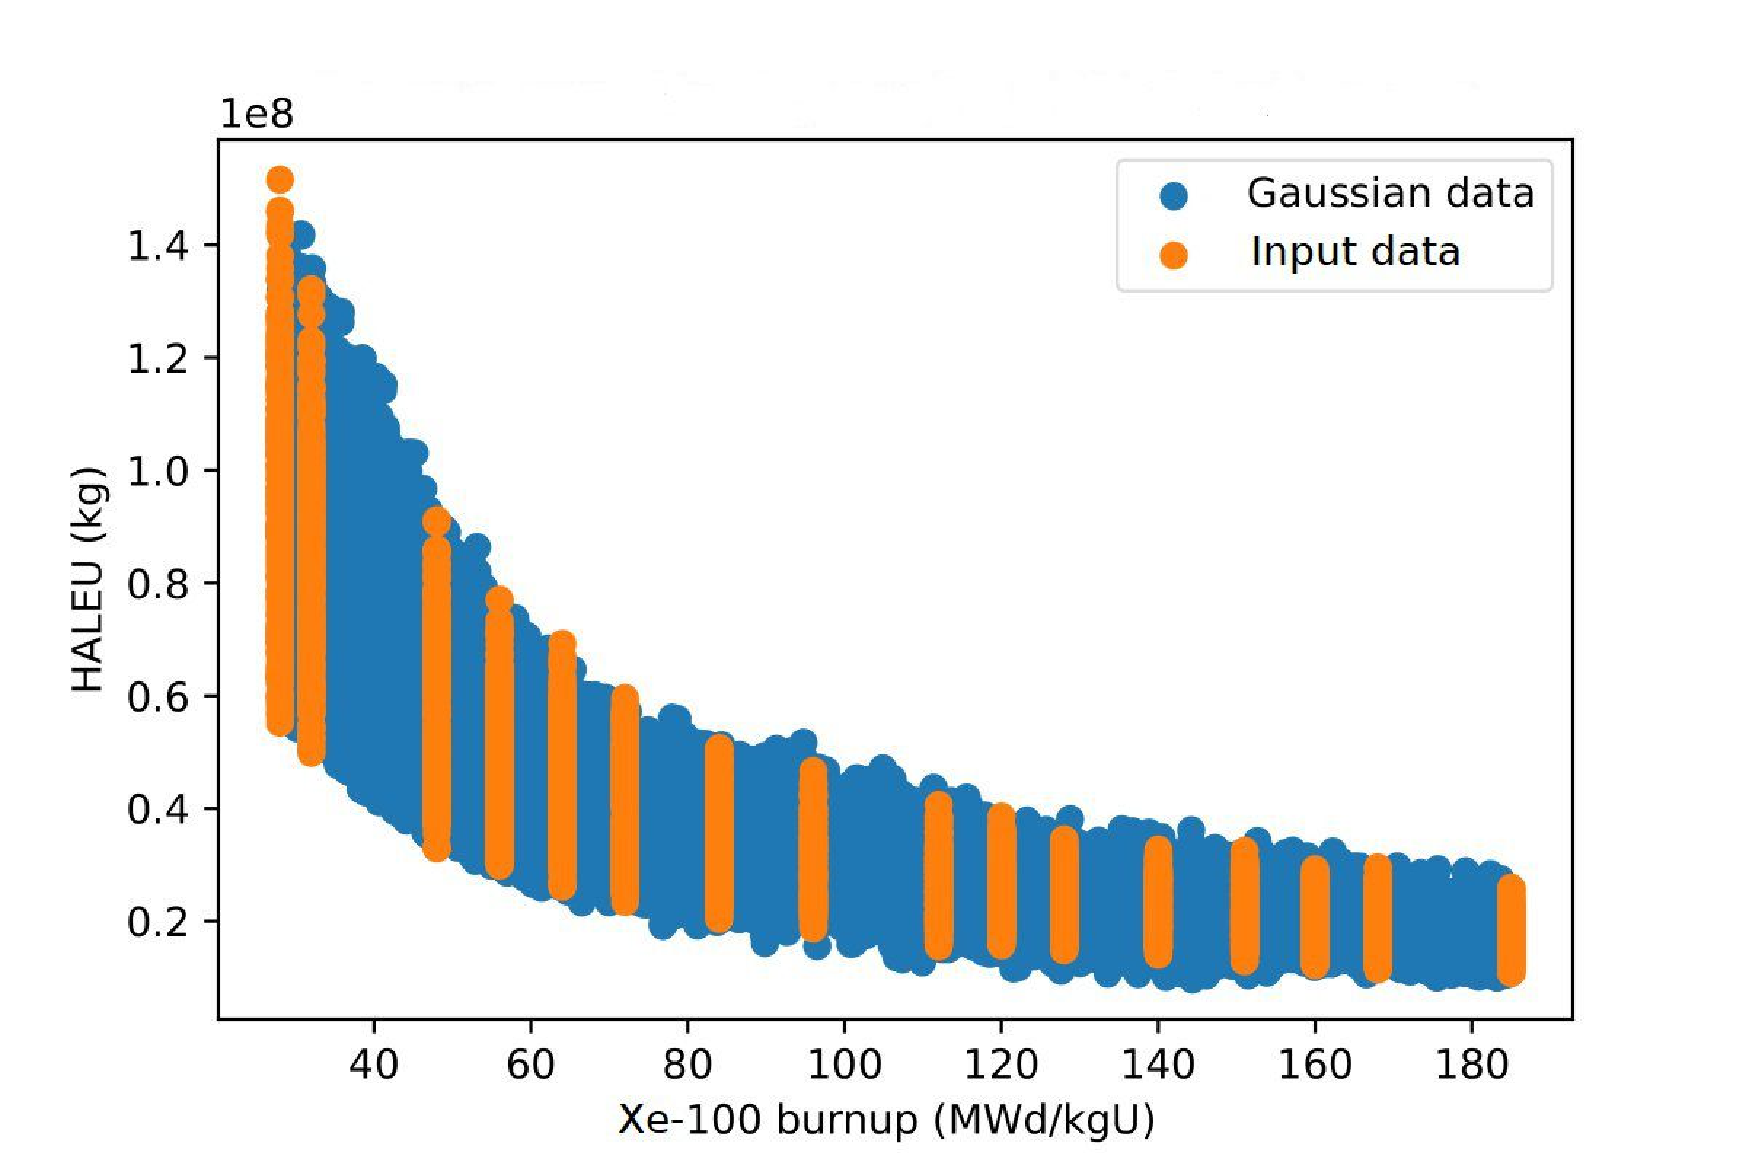
\includegraphics[scale=0.8]{voygr_share_gaussian_xe100_burnup_haleu.pdf}
    \caption{Comparison of the input data and the results of the Gaussian 
    surrogate model when the VOYGR build share is varied.}
    \label{fig:s7_voygr_gaussian}
\end{figure}

The Sobol' indices from this model, shown in Table \ref{tab:s7_sobol_voygr_gaussian}
show a similar trend to the Sobol' indices from varying the \gls{MMR}
build share. The Xe-100 burnup has the largest impact on all of the 
results, the transition start time and \gls{MMR} burnup have no 
effect on the metrics, and the \gls{LWR} lifetimes and VOYGR build share 
have a very small impact on the metrics. 

Based on the results of 
the \gls{OAT} analysis, increasing the VOYGR build share replaces 
Xe-100s with VOYGRs. Therefore, the VOYGR build share implicitly 
impacts the Xe-100 build share, which leads to this input parameter 
having a larger impact on the metrics than most of the other variables. 
The VOYGR build share has a larger impact on the fuel mass and the 
\gls{SNF} mass than the other metrics because the VOYGR takes in more 
and discharges more 
fuel than the Xe-100 and \gls{MMR} per unit time and energy. The 
increased impact of the VOYGR build share on these metrics leads to 
the decreased impact of the Xe-100 burnup, relative to the 
\gls{HALEU}-related metrics. 

\begin{table}
    \centering
    \caption{Sobol' indices for the Gaussian model when varying the VOYGR 
    build share. The first number is the main index, the second is the total 
    index.}
    \label{tab:s7_sobol_voygr_gaussian}
    \begin{tabular}{c c c c c c c}
        \hline
        & \multicolumn{6}{c}{Output Metric} \\
        Parameter & Fuel Mass & HALEU Mass & SWU & HALEU SWU & Feed & SNF Mass \\
        \hline
        Transition Start & 0.002/0.003 & 0.000/0.001 & 0.000/0.002 & 
                           0.000/0.001 & 0.000/0.001 & 0.001/0.003\\
        LWR Lifetime & 0.065/0.076 & 0.020/0.033 & 0.033/0.045 & 
                       0.020/0.033 & 0.020/0.033 & 0.069/0.081\\
        VOYGR Build Share & 0.252/0.284 & 0.114/0.0151 & 0.028/0.067 &
                            0.114/0.151 & 0.114/0.151 & 0.204/0.238\\
        Xe-100 Burnup & \cellcolor{green!25}0.652/0.683 & \cellcolor{green!25}0.837/0.883 & \cellcolor{green!25}0.910/0.956 & 
        \cellcolor{green!25}0.836/0.881 & \cellcolor{green!25}0.836/0.881 & \cellcolor{green!25}0.696/0.730\\
        MMR Burnup & 0.002/0.002 & 0.000/0.002 & 0.001/0.001 & 
                     0.001/0.002 & 0.001/0.002 & 0.002/0.002\\
        \hline        
    \end{tabular}
\end{table}

When using the quadratic fit, the R$^2$ values range between 0.94-0.95. 
These values are consistent with the R$^2$ values for the other 
quadratic models in this work. The data from this quadratic model,
compared with the input data in Figure \ref{fig:s7_voygr_quadratic}, 
shows that it does not fully reach the maximum of the input data
and under-predicts some of the minimum values. These trends have 
been observed in all of the quadratic models created for this analysis. 

\begin{figure}
    \centering 
    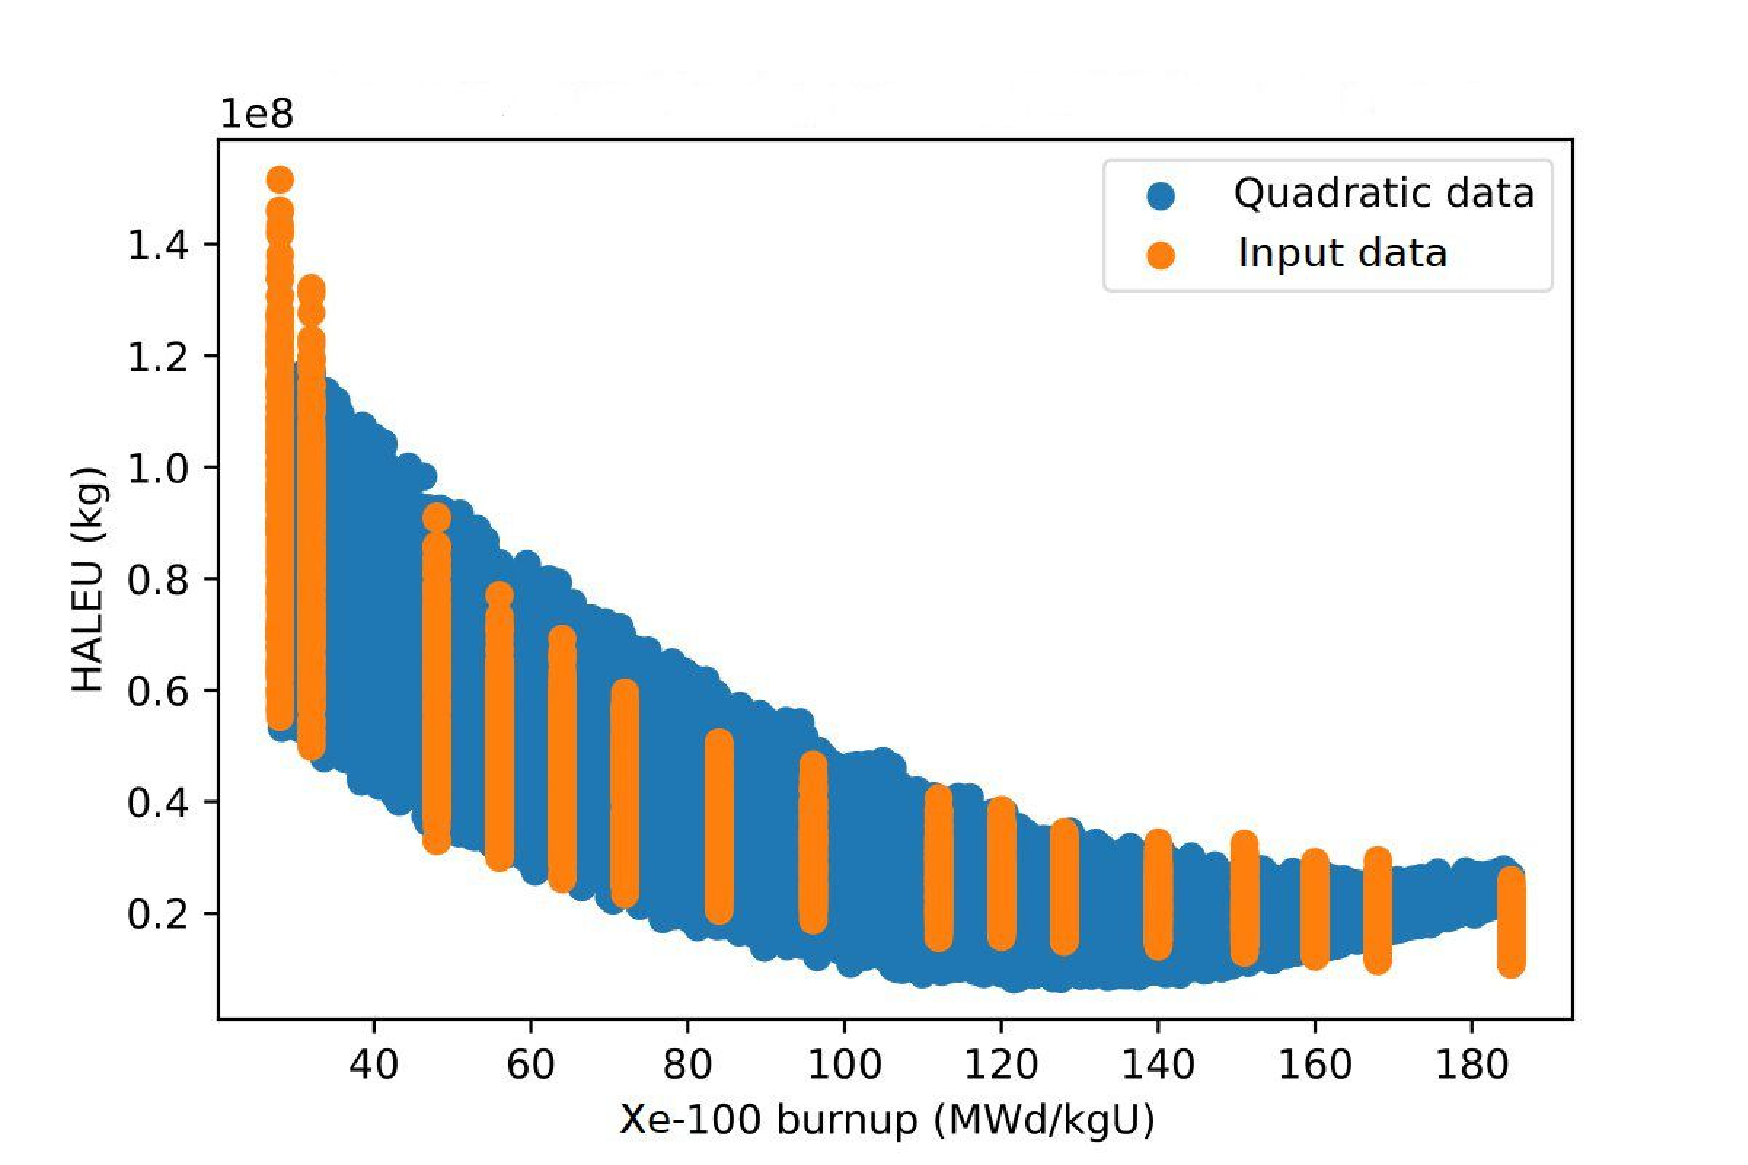
\includegraphics[scale=0.8]{voygr_share_quadratic_xe100_burnup_haleu.pdf}
    \caption{Comparison of the input data and the results of the quadratic 
    surrogate model when the VOYGR build share is varied.}
    \label{fig:s7_voygr_quadratic}
\end{figure}

The Sobol' indices from this model, given in Table \ref{tab:s7_sobol_voygr_quadratic},
have the same pattern as the Sobol' indices from the Gaussian model created. 
This data does not provide any new insights into how each input parameter
affects the output metrics of this transition scenario. 

\begin{table}
    \centering
    \caption{Sobol' indices for the quadratic model when varying the VOYGR 
    build share. The first number is the main index, the second is the total 
    index.}
    \label{tab:s7_sobol_voygr_quadratic}
    \begin{tabular}{c c c c c c c}
        \hline
        & \multicolumn{6}{c}{Output Metric} \\
        Parameter & Fuel Mass & HALEU Mass & SWU & HALEU SWU & Feed & SNF Mass \\
        \hline
        Transition Start & 0.002/0.002 & 0.000/0.000 & 0.000/0.001 &
                           0.000/0.000 & 0.000/0.000 & 0.001/0.002\\
        LWR Lifetime & 0.063/0.071 & 0.020/0.031 & 0.031/0.042 &
                       0.051/0.031 & 0.020/0.031 & 0.066/0.075\\
        VOYGR Build Share & 0.214/0.243 & 0.108/0.143 & 0.030/0.066 &
                            0.108/0.143 & 0.108/0.143 & 0.170/0.200\\
        Xe-100 Burnup & \cellcolor{green!25}0.700/0.724 & \cellcolor{green!25}0.843/0.884 & \cellcolor{green!25}0.911/0.952 &
        \cellcolor{green!25}0.842/0.883 &\cellcolor{green!25} 0.843/0.883 & \cellcolor{green!25}0.740/0.767\\
        MMR Burnup & 0.001/0.001 & 0.001/0.001 & 0.001/0.002 &
                     0.001/0.002 & 0.001/0.001 & 0.001/0.001\\
        \hline        
    \end{tabular}
\end{table}


\subsection{Scenario 14}
